\chapter{Multi-agent refinement quantified modal logic}\label{k}

In this chapter we will provide a sound and complete axiomatisation of the
multi-agent refinement quantified modal logic, over the class of \classK{}. 

\section{Technical preliminaries}

The axiomatisation of the single-agent refinement quantified modal logic given
by van Ditmarsch, French and Pinchinat~\cite{french2010future} relied on a
disjunctive normal form defined in terms of the cover operator, $\covers$. We
introduce the same disjunctive normal form for our result in multi-agent
refinement quantified modal logic, as we will be using a similar provably
correct translation in order to show the completeness of our axiomatisation.

\begin{definition}[Disjunctive normal form]
A formula in disjunctive normal form is defined by the following abstract syntax:
$$
\alpha ::= \pi \land \bigwedge_{a \in B} \covers_a \Gamma_a \bnfalt \alpha \lor \alpha
$$
where $\pi$ stands for a propositional formula, $B \subseteq A$, and for $a \in
B$, $\Gamma_a$ stands for a finite set of formulae in disjunctive normal form.
\end{definition}

To show that every \lang{} formula is equivalent to a disjunctive normal
formula, we first introduce the negation normal form and a corresponding lemma
for that form.

\begin{definition}[Negation normal form]
A formula in negation normal form is defined by the following abstract syntax:
$$
\alpha ::= p \bnfalt 
\neg p \bnfalt
\alpha \land \alpha \bnfalt
\alpha \lor \alpha \bnfalt
\knows_a \alpha \bnfalt
\suspects_a \alpha
$$
where $p \in P$ and $a \in A$.
\end{definition}

\begin{lemma}\label{k-nnf}
Every formula of \lang{} is equivalent to a formula in negation normal form,
under the semantics of \logicK{}.
\end{lemma}

\begin{proof}
Similar to negation normal forms in propositional logic, we can recursively push
the negations inwards using the following equivalences:
\begin{eqnarray*}
\neg \neg \phi &\iff& \phi\\
\neg (\phi \land \psi) &\iff& \neg \phi \lor \neg \psi\\
\neg \knows_a \phi &\iff& \suspects_a \neg \phi
\end{eqnarray*}
\end{proof}

\begin{lemma}\label{k-dnf}
Every formula of \lang{} is equivalent to a formula in disjunctive normal form,
under the semantics of \logicK{}.
\end{lemma}

\begin{proof}
Let $\alpha \in \lang$. Without loss of generality, by Lemma~\ref{k-nnf}, we may
assume that $\alpha$ is in negation normal form. We prove by induction over the
structure of $\alpha$ that $\alpha$ is equivalent to a formula in disjunctive
normal form. The induction hypothesis is that every strict subformula of
$\alpha$ has an equivalent in disjunctive normal form.

The base case is when $\alpha = p$ or $\alpha = \neg p$ for some $p \in P$, in
which case we are done.

Suppose that $\alpha = \phi \lor \psi$. By the induction hypothesis, there are
formulae $\phi'$ and $\psi'$ in disjunctive normal form that are equivalent to
$\phi$ and $\psi$ respectively. Then $\phi \lor \psi \iff \phi' \lor \psi'$,
which is in disjunctive normal form.

Suppose that $\alpha = \knows_a \phi$. By the induction hypothesis, there is a
formula $\phi'$ in disjunctive normal form that is equivalent to $\phi$. Then
$\knows_a \phi \iff \covers_a \{\phi\} \lor \covers_a \emptyset$, which is in
disjunctive normal form.

Suppose that $\alpha = \suspects_a \phi$. By the induction hypothesis, there is
a formula $\phi'$ in disjunctive normal form that is equivalent to $\phi$. Then
$\suspects_a \phi \iff \covers_a \{\phi, \top\}$, which is in disjunctive normal
form.

Suppose that $\alpha = \phi \land \psi$. By the induction hypothesis, there are
formulae $\phi'$ and $\psi'$ in disjunctive normal form that are equivalent to
$\phi$ and $\psi$ respectively. Then $\phi \land \psi \iff \phi' \land \psi'$.
As $\phi'$ and $\psi'$ are in disjunctive normal form, then $\phi' = \delta_1
\lor \cdots \lor \delta_m$ and $\psi' = \gamma_1 \lor \cdots \lor \gamma_m$ for
some $m, n \geq 0$, where each of the $\delta_i$ and $\gamma_i$ are terms of the
form $\pi \land \bigwedge_{a \in B \subseteq A} \covers_a \Gamma_a$.  Then we
can rewrite $\alpha$ as a disjunction of conjunctions, by the following
equivalence:
$$
\phi' \land \psi' \iff \bigvee_{i \leq m, j \leq n} \delta_i \land \gamma_j
$$

For each $i \leq m$ and $j \leq n$, we have that $\delta_i = \pi \land
\bigwedge_{a \in B \subseteq A} \covers_a \Gamma_a$, and $\gamma_j = \rho \land
\bigwedge_{a \in C \subseteq A} \covers_a \Gamma'_a$, where $\pi$ and $\rho$ are
propositional formulae, and each $\Gamma_a$ and $\Gamma'_a$ is a set of
disjunctive normal formulae. Then we can write each conjunction as: 
$$\delta_i \land \gamma_i \iff (\pi \land \rho) \land \bigwedge_{a \in B
\subseteq A} \covers_a \Gamma_a \land \bigwedge_{a \in C \subseteq A} \covers_a
\Gamma'_a$$

We note that the sets of agents $B$ and $C$ may intersect, and hence the same
agent may appear in each of those sets, possibly with different sets of formulae
$\Gamma_a$ and $\Gamma'_a$. We can combine the two sets of formulae into one, so
that each agent appears only once, using the following equivalence:
$$
\covers_a \Gamma \land \covers_a \Gamma' \equiv 
\covers_a \big( 
\{ \gamma \land \bigvee_{\gamma' \in \Gamma'} \gamma' \mid \gamma \in \Gamma \}
\cup
\{ \gamma' \land \bigvee_{\gamma \in \Gamma} \gamma \mid \gamma' \in \Gamma' \}
\big)
$$
We note that as each $\gamma \in \Gamma$ and $\gamma' \in \Gamma'$ are assumed
to be disjunctive normal formulae, that applying a disjunction over each of
these sets yields a disjunctive normal formula. Conjoining two disjunctive
normal formulae does not yield a disjunctive normal formula, however an
inductive argument can be used to show that recursively applying the same
translation described here, to each of these conjunctions, yields a disjunctive
normal formula.

Repeating this for each disjunct in our original formula leaves us with a
formula in cover logic disjunctive normal form.

Therefore every formula of \lang{} is equivalent to a formula in disjunctive
normal form.
\end{proof}

We note that, similar to disjunctive normal forms in propositional logic, and to
the prenex normal form introduced for the single-agent doxastic and epistemic
logics, conversion into disjunctive normal form in modal logic can result
in a formula that is exponentially larger than the original formula in the worst
case.

\pagebreak
\section{Axiomatisation}

We provide an axiomatisation of the multi-agent refinement quantified modal
logic, \logicKF{}, and prove its soundness and completeness.
\begin{definition}[Axiomatisation \axiomKF]
The axiomatisation \axiomKF{} is a substitution schema consisting of the
following axioms:
$$
\begin{array}{rl}
{\bf P} & \text{All propositional tautologies}\\
{\bf K} & \knows (\phi \implies \psi) \implies \knows \phi \implies \knows
\psi\\
{\bf R} & \allrefs_a (\phi \implies \psi) \implies \allrefs_a \phi \implies
\allrefs_a \psi\\
{\bf RP} & \allrefs_a \alpha \iff \alpha \text{ where $\alpha$ is a
propositional formula}\\
{\bf RComm} & \displaystyle \somerefs_a \covers_b \Gamma \iff \covers_b \{\somerefs_a \gamma
\mid \gamma \in \Gamma\} \text{ where $a \neq b$}\\
{\bf RDist} & \displaystyle \bigwedge_{b \in B} \somerefs_a \covers_b \Gamma_b \implies
\somerefs_a \bigwedge_{b \in B} \covers_b \Gamma_b \text{ where $B \subseteq A$}\\
{\bf RK} & \displaystyle \somerefs_a \covers_a \Gamma \iff \bigwedge_{\gamma \in \Gamma}
\suspects_a \somerefs_a \gamma\\
\end{array}
$$

Along with the rules:
$$
\begin{array}{rl}
{\bf MP} & \text{From $\proves \phi \implies \psi$ and $\proves \phi$, infer
$\proves \psi$}\\
{\bf NecK} & \text{From $\proves \phi$ infer $\proves \knows_a \phi$}\\
{\bf NecR} & \text{From $\proves \phi$ infer $\proves \allrefs_a \phi$}
\end{array}
$$
\end{definition}

The axiomatisation \axiomKF{} shares many of the axioms and rules of the
axiomatisation from the single-agent case. The axioms {\bf P}, {\bf K}, {\bf R},
{\bf RP} and {\bf RK}, and the rules {\bf MP}, {\bf NecK} and {\bf NecR} are
essentially the same as the axioms that van Ditmarsch, French and
Pinchinat~\cite{french2010future} used in the single-agent case. The differences
are that \axiomKF{} contains axioms for handling the interaction between
multiple agents. The axioms {\bf RComm} and {\bf RDist} are novel axioms used to
handle the situation where a refinement quantifier is applied to a cover
operator of a different agent, and where a refinement quantifier is applied to a
conjunction of cover operators belonging to different agents. We call these
axioms {\bf RComm} and {\bf RDist} because they correspond to properties that
are visually similar to commutativity or distributivity of the $\somerefs$
opereator over the $\covers$ operators for different agents.

\begin{example}\label{k-example}
We give an example derivation using \axiomKF{}, based on the coin-flipping
example given in Example~\ref{semantics-coin-s5}. We suppose that neither Alice
nor Bob know whether the coin has landed on heads or tails, and we show that it
is possible for Alice to learn that the coin landed on heads, whilst Bob
continues to not know. Thus we give a derivation of $(\neg \knows_a p \land \neg
\knows_a \neg p \land \neg \knows_b p \land \neg \knows_b \neg p) \implies
\somerefs_a (\knows_a p \land \neg \knows_b p)$. Let $\phi = \neg \knows_a p \land \neg
\knows_a \neg p \land \neg \knows_b p \land \neg \knows_b \neg p$.
$$
\begin{array}{ll}
\proves \phi \implies \neg
\knows_a \neg p \land \neg \knows_b p & \text{({\bf P})}\\
\proves \phi \implies
\suspects_a p \land \suspects_b \neg p & \text{(Definition of $\suspects$)}\\
\proves \phi \implies
\suspects_a p \land \covers_b \{\neg p, \top\} & \text{(Definition of $\covers$)}\\
\proves \phi \implies
\suspects_a \neg \neg p \land \covers_b \{\neg \neg \neg p, \neg \neg \top\} &
\text{({\bf P})}\\
\proves \phi \implies
\suspects_a \neg \allrefs_a \neg p \land \covers_b \{\neg \allrefs_a \neg \neg
p, \neg \allrefs_a \neg \top\} & \text{({\bf RP})}\\
\proves \phi \implies
\suspects_a \somerefs_a p \land \covers_b \{\somerefs_a \neg
p, \somerefs_a \top\} & \text{(Definition of $\somerefs$)}\\
\proves \phi \implies
\somerefs_a \covers_a \{p\} \land \covers_b \{\somerefs_a \neg
p, \somerefs_a \top\} & \text{({\bf RK})}\\
\proves \phi \implies
\somerefs_a \covers_a \{p\} \land \somerefs_a \covers_b \{\neg
p, \top\} & \text{({\bf RComm})}\\
\proves \phi \implies
\somerefs_a (\covers_a \{p\} \land \covers_b \{\neg
p, \top\}) & \text{({\bf RDist})}\\
\proves \phi \implies
\somerefs_a (\knows_a p \land \suspects_b \neg
p) & \text{(Definition of $\covers$)}\\
\proves \phi \implies
\somerefs_a (\knows_a p \land \knows_b p) & \text{(Definition of $\suspects$)}\\
\end{array}
$$
\end{example}

We will now show that the axiomatisation is sound with respect to \classK{}
models.

\begin{lemma}\label{k-sound}
The axiomatisation \axiomKF{} is sound with respect to the semantic class
\classK{}.
\end{lemma}

\begin{proof}
The soundness of the axioms {\bf P} and {\bf K}, and the rules {\bf MP} and
{\bf NecK} can be shown by the same reasoning used to show that they are sound
in basic modal logic. As the axioms {\bf RP} and {\bf R}, and the rule {\bf
NecR} involve only a single agent, their soundness can be shown by the same
reasoning used to show that they are sound in the single-agent refinement
quantified modal logic~\cite{french2010future}.

All that remains to be shown is the soundness of {\bf RK}, {\bf RComm}, and {\bf
RDist}.

\paragraph{RK}
Suppose that $M_s \in \classK$ is a Kripke model such that $M_s \entails
\bigwedge_{\gamma \in \Gamma} \suspects_a \somerefs_a \gamma$.

We need to show that $M_s \entails \somerefs_a \covers_a \Gamma$. To do this we
will construct a model $N_t \in \classK$, construct an $a$-simulation from $N_t$
to $M_s$ to show that $N_t \refinement_a M_s$, and finally show that $N_t
\entails \covers_a \Gamma$.

We begin by constructing the model $N_t$. Consider $\gamma \in \Gamma$. From
$M_s \entails \suspects_a \somerefs_a \gamma$, there exists a state $s^\gamma
\in sR^M$ such that $M_{s^\gamma} \entails \somerefs_a \gamma$. Therefore there
exists a Kripke model $N^\gamma_{t^\gamma} \refinement_a M_{s^\gamma}$, via some
$a$-simulation $\mathcal{R}^\gamma$, such that $N^\gamma_{t^\gamma} \entails
\gamma$. Without loss of generality we assume that the $N^\gamma$ are disjoint.

Let $t$ be a state not in $S^M$ or any of the $S^{N^\gamma}$. Then we construct a
Kripke model $N = (S^N, R^N, V^N)$ where:
\begin{eqnarray*}
S^N &=& \{t\} \cup S^M \cup \bigcup_{\gamma \in \Gamma} S^{N^\gamma}\\
R^N_a &=& \{(t, t^\gamma) \mid \gamma \in \Gamma\}
\cup R^M_a
\cup \bigcup_{\gamma \in \Gamma} R^{N^\gamma}_a\\
R^N_b &=& \{(t, t') \mid t' \in sR^M_b\}
\cup R^M_b
\cup \bigcup_{\gamma \in \Gamma} R^{N^\gamma}_b \text{ for $b \in A - \{a\}$}\\
V^N(p) &=& 
\begin{cases}
\displaystyle \{t\} \cup V^M(p) \cup \bigcup_{\gamma \in \Gamma} V^{N^\gamma}(p) & \text{if $s
\in V^M(p)$}\\
\displaystyle V^M(p) \cup \bigcup_{\gamma \in \Gamma} V^{N^\gamma}(p) & \text{otherwise}
\end{cases}
\text{ for $p \in P$}
\end{eqnarray*}

A representation of this model is pictured in Figure~\ref{k-diagram}.

\begin{figure}
\begin{center}
\scalebox{0.4}{
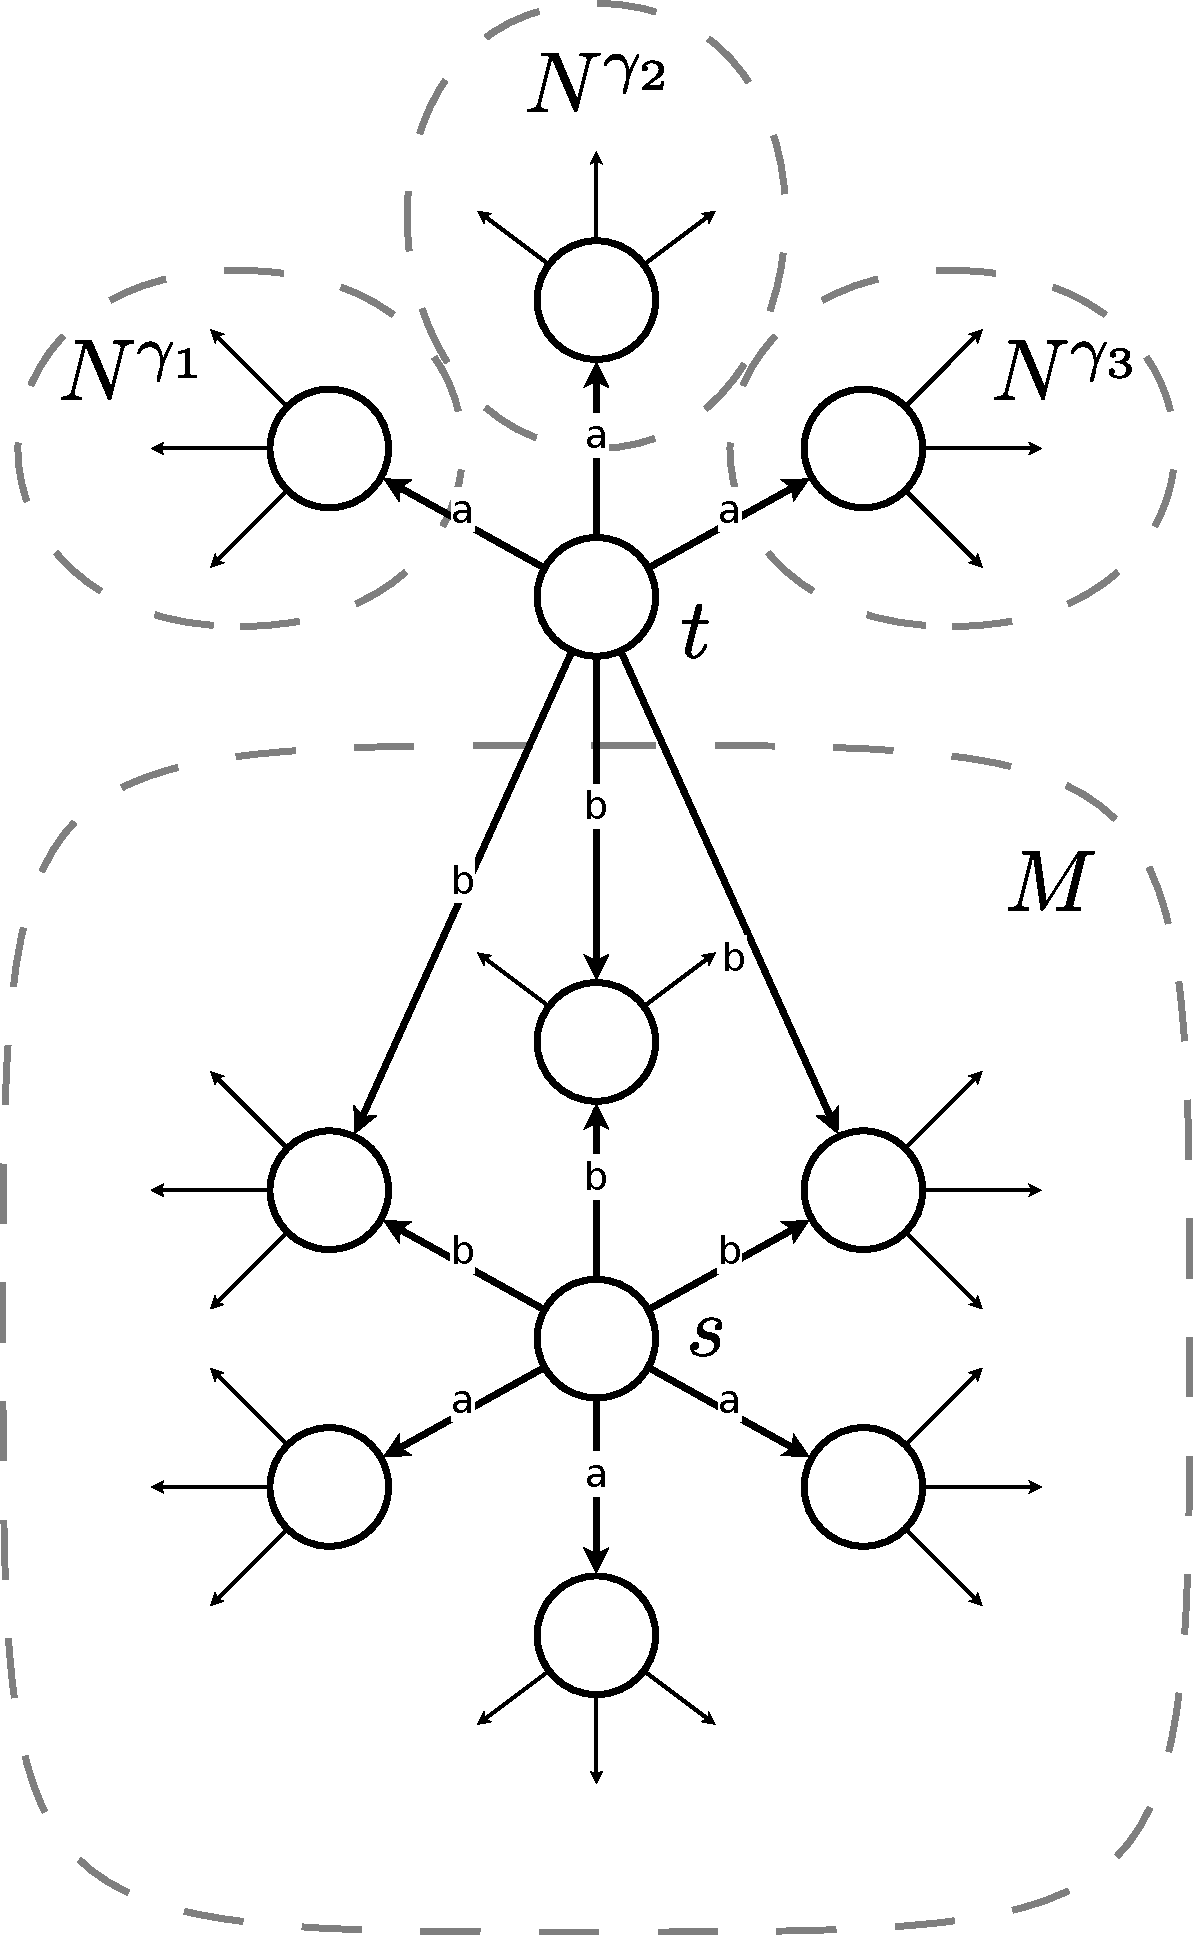
\includegraphics{rk}
}
\caption{\label{k-diagram}
The model $N$ is constructed by taking the model $M$ and the models $N^\gamma$
for every $\gamma \in \Gamma$, and connecting them with an extra node $t$. $t$
is connected via an $a$-edge to $t^\gamma$ from each of the $N^\gamma$, and is
also connected via a $b$-edge to each $b$-successor of $s$ in $M$. $N_t$ is
then the desired $a$-refinement of $M_s$.
}
\end{center}
\end{figure}

We construct an $a$-simulation $\mathcal{R}$ from $N_t$ to $M_s$, where:
$$\mathcal{R} = \{(t, s)\} \cup \{(s', s') \mid s' \in S^M \} 
\cup \bigcup_{\gamma \in \Gamma} \mathcal{R}^\gamma$$

We must show that $\mathcal{R}$ satisfies {\bf atoms}, {\bf forth-$b$} for every
$b \in A$, and {\bf back-$b$} for every $b \in A - \{a\}$.

\paragraph{atoms} We note that, by construction, the valuation of $N$ matches
the valuation of its corresponding states in $M$ and each $N^\gamma$, and the
valuation of $N_t$ matches that of $M_s$. Therefore $\mathcal{R}$ satisfies {\bf
atoms}.

\paragraph{forth} We next show that $\mathcal{R}$ satisfies {\bf forth-$b$} for
every $b \in A$.  Let $b \in A$ and let $(u, v) \in \mathcal{R}$.

Suppose that $(u, v) \in \mathcal{R}^\gamma$ for some $\gamma \in \Gamma$.  Then
as $\mathcal{R}^\gamma$ is an $a$-simulation, it satisfies {\bf forth-$b$} for
every $b \in A$. Hence for every $u' \in uR^{N^\gamma}_b = uR^N_b$, there exists
some $v' \in vR^M_b$ such that $(u', v') \in \mathcal{R}^\gamma \subseteq
\mathcal{R}$. 

Suppose instead that $(u, v) = (s', s')$ for some $s' \in S^M$.  Then we note
that $s'R^N_b = s'R^M_b$, and hence for every $s'' \in s'R^N_b$ we have that
$s'' \in s'R^M_b$, and that $(s'', s'') \in \mathcal{R}$. 

Finally suppose that $(u, u') = (t, s)$. We must consider the cases where $b =
a$ and where $b \neq a$. So suppose that $b = a$. By construction, $tR^N_a =
\{t^\gamma \mid \gamma \in \Gamma\}$, and hence $v = t^\gamma$ for some $\gamma
\in \Gamma$. Hence we can take $s^\gamma \in sR^M_a$, and note that as
$\mathcal{R}^\gamma$ is an $a$-simulation from $M_{s^\gamma}$ to
$N^\gamma_{t^\gamma}$, we know that $(t^\gamma, s^\gamma) \in \mathcal{R}^\gamma
\subseteq \mathcal{R}$. Suppose that $b \neq a$. Then by construction, $tR^M_b =
sR^M_b$, hence for every $t' \in tR^M_b$, we have that $t' \in sR^M_b$, and
hence we know that $(t', t') \in \mathcal{R}$. 

Therefore $\mathcal{R}$ satisfies {\bf forth-$b$} for every $b \in A$.

\paragraph{back} A similar argument to the above shows that $\mathcal{R}$
satisfies {\bf back-$a$} for every $b \in A - \{a\}$.

Therefore $\mathcal{R}$ is an $a$-simulation, and $N_t \refinement_a M_s$.

Finally we show that $N_t \entails \covers_a \Gamma$. We must show that for each
$\gamma \in \Gamma$ that $N_{t^\gamma} \entails \gamma$. This follows from the
fact that $N_{t^\gamma}$ is bisimilar to $N^\gamma_{t^\gamma}$. This is obvious,
as $N$ contains a duplicate of $N^\gamma$, and $N$ does not add any additional
edges originating from states in $S^{N^\gamma}$. Hence from bisimulation
invariance, $N_{t^\gamma} \entails \gamma$ for every $\gamma \in \Gamma$, and
hence $N_t \entails \covers_a \Gamma$.

As $N_t \refinement_a M_s$, and $N_t \entails \covers_a \Gamma$ we therefore
have that $M_s \entails \somerefs_a \covers_a \Gamma$.

Conversely, suppose that $M_s \entails \covers_a \Gamma$. Then there exists a
Kripke model $N_t \refinement_a M_s$, via some $a$-simulation $\mathcal{R}$,
such that $N_t \entails \covers_a \Gamma$. From the definition of the cover
operator, this implies that $N_t \entails \knows_a \bigvee_{\gamma \in \Gamma}
\gamma \land \bigwedge_{\gamma \in \Gamma} \suspects_a \gamma$. In particular we
note that for every $\gamma \in \Gamma$, $N_t \entails \suspects_a \gamma$, and
so there exists some $t^\gamma \in tR^N_a$ such that $N_{t^\gamma} \entails
\gamma$. As $t^\gamma \in tR^N_a$, and $(t, s) \in \mathcal{R}$, by {\bf
forth-$a$} there exists some $s^\gamma \in sR^M_a$ such that $(t^\gamma, s^\gamma)
\in \mathcal{R}$. Hence $\mathcal{R}$ is also an $a$-simulation from
$N_{t^\gamma}$ to $M_{s^\gamma}$, and so $M_{s^\gamma} \entails \somerefs_a
\gamma$. As for every $\gamma \in \Gamma$ we have that $s^\gamma \in sR^M_a$, we
also have that $M_s \entails \suspects_a \somerefs_a \gamma$. Therefore we
finally have that $M_s \entails \bigwedge_{\gamma \in \Gamma} \suspects_a
\somerefs_a \gamma$.

Therefore {\bf RK} is sound.

\paragraph{RComm}
Suppose that $M_s \in \classK$ is a Kripke model such that $M_s \entails
\covers_b \{ \somerefs_a \gamma \mid \gamma \in \Gamma\}$, where $a \neq b$.

We need to show that $M_s \entails \somerefs_a \covers_b \Gamma$. To do this we
follow the same strategy as for proving {\bf RK}: we construct an $a$-refinement
$N_t \in \classK$, and show that $N_t \entails \covers_b \Gamma$.

We begin by constructing the model $N_t$. Consider $\gamma \in \Gamma$. From
$M_s \entails \covers_b \{ \somerefs_a \gamma \mid \gamma \in \Gamma \}$, there
exists a state $s^\gamma \in sR^M_b$ such that $M_{s^\gamma} \entails
\somerefs_a \gamma$. Therefore there exists a Kripke model $N^\gamma_{t^\gamma}
\refinement_a M_{s^\gamma}$, via some $a$-simulation $\mathcal{R}^\gamma$, such
that $N^\gamma_{t^\gamma} \entails \gamma$. Without loss of generality we assume
that the $N^\gamma$ are disjoint.

Let $t$ be a state not in $S^M$ or any of the $S^{N^\gamma}$. Then we construct a
Kripke model $N = (S^N, R^N, V^N)$ where:
\begin{eqnarray*}
S^N &=& \{t\} \cup S^M \bigcup_{\gamma \in \Gamma} S^{N^\gamma}\\
R^N_b &=& \{(t, t^\gamma) \mid \gamma \in \Gamma\} 
\cup  R^M_b 
\cup \bigcup_{\gamma \in \Gamma} R^{N^\gamma}_b\\
R^N_c &=& \{(t, t') \mid t' \in sR^M_c\} 
\cup R^M_c \cup \bigcup_{\gamma \in \Gamma} R^{N^\gamma}_c \text{ for $c \in A - \{b\}$}\\
V^N(p) &=& 
\begin{cases}
\displaystyle \{t\} \cup V^M(p) \cup \bigcup_{\gamma \in \Gamma} V^{N^\gamma}(p)
& \text{if $s \in V^M(p)$}\\
\displaystyle V^M(p) \cup \bigcup_{\gamma \in \Gamma} V^{N^\gamma}(p) &
\text{otherwise}
\end{cases}
\text{ for $p \in P$}
\end{eqnarray*}

We construct an $a$-simulation $\mathcal{R}$ from $N_t$ to $M_s$, where:
$$\mathcal{R} = \{(t, s)\} \cup \{(s', s') \mid s' \in S^M\} \cup
\bigcup_{\gamma \in \Gamma} \mathcal{R}^\gamma$$

We note that $\mathcal{R}$ is an $a$-simulation, by similar arguments as used in
the proof for {\bf RK}. In particular, this means that $N_t \refinement_a M_s$.

We also note that for every $\gamma \in \Gamma$, that $N_{t^\gamma} \entails
\gamma$, by similar arguments as used in the proof for {\bf RK}. In particular,
this means that $N^\gamma_t \entails \covers_b \Gamma$.

Therefore $M_s \entails \somerefs_a \covers_b \Gamma$.

The converse, $\somerefs_a \covers_b \Gamma \implies \covers_b \{\somerefs_a
\gamma \mid \gamma \in \Gamma\}$ follows a similar proof to the relevant part in
the proof for {\bf RK}.

Therefore {\bf RComm} is sound.

\paragraph{RDist}
Suppose that $M_s \in \classK$ is a Kripke model such that $M_s \entails
\bigwedge_{b \in B} \somerefs_a \covers_b \Gamma_b$, where $B \subseteq A$.

We need to show that $M_s \entails \somerefs_a \bigwedge_{b \in B} \covers_b
\Gamma_b$. To do this we follow the same strategy as for proving {\bf RK}: we
construct an $a$-refinement $N_t \in \classK$, and show that $N_t \entails
\somerefs_a \bigwedge_{b \in B} \covers_b \Gamma_b$.

We begin by constructing the model $N_t$. Suppose that $a \in B$. Then we have
$M_s \entails \somerefs_a \covers_a \Gamma_a$, and by {\bf RK} this implies that
$M_s \entails \bigwedge_{\gamma \in \Gamma_a} \gamma$. We also have that for
every $b \in B - \{a\}$ that $M_s \entails \somerefs_a \covers_a \Gamma_b$, and
by {\bf RComm} this implies that $M_s \entails \covers_b \{\somerefs_a \gamma
\mid \gamma \in \Gamma_b\}$, and by the definition of the cover operator, this
implies that $M_s \entails \bigwedge_{\gamma \in \Gamma_b} \suspects_b
\somerefs_a \gamma$. Hence for every $b \in B$ and $\gamma \in \Gamma_b$, we
have that $\suspects_b \somerefs_a \gamma$. This implies that for each $b \in B$
and each $\gamma \in \Gamma_b$ that there exists some $s^{b,\gamma} \in sR^M_b$ such
that $M_{s^{a,\gamma}} \entails \somerefs_a \gamma$. Therefore there exists a Kripke
model $N^{b,\gamma}_{t^{b,\gamma}} \refinement_a M_{s^{a,\gamma}}$ such that
$N^{b,\gamma}_{t^{b,\gamma}} \entails \gamma$. Without loss of generality we
may assume that the $N^{b,\gamma}$ are disjoint.

Let $t$ be a state not in $S^M$ or any of the $S^{N^{b,\gamma}}$. Then we construct a
Kripke model $N = (S^N, R^N, V^N)$ where:
\begin{eqnarray*}
S^N &=& \{t\} \cup S^M \cup \bigcup_{b \in A, \gamma \in \Gamma_b} S^{N^{b,\gamma}}\\
R^N_b &=& \{(t, t^{b,\gamma}) \mid \gamma \in \Gamma_b\} \cup R^M_b \cup
\bigcup_{c \in B, \gamma \in \Gamma_c} R^{N^{c,\gamma}}_b \text{ for $b \in
B$}\\
R^N_b &=& \{(t, t') \mid t' \in sR^M_b\} \cup R^M_b \cup
\bigcup_{c \in B, \gamma \in \Gamma_c} R^{N^{c,\gamma}}_b \text{ for $b \in A
\setminus B$}\\
V^N(p) &=& 
\begin{cases}
\displaystyle \{t\} \cup V^M(p) \cup \bigcup_{b \in B, \gamma \in \Gamma_b}
V^{N^{b,\gamma}}(p) & \text{if $s \in V^M(p)$}\\
\displaystyle V^M(p) \cup \bigcup_{b \in B, \gamma \in \Gamma_b}
V^{N^{b,\gamma}}(p) & \text{otherwise}
\end{cases}
\end{eqnarray*}

We construct an $a$-simulation $\mathcal{R}$ from $N_t$ to $M_s$, where:
$$\mathcal{R} = \{(t, s)\} \cup \{(s', s') \mid s' \in S^M\} \bigcup_{b \in A,
\gamma \in \Gamma_b} \mathcal{R}^\gamma$$

We note that this is an $a$-simulation, by similar arguments as used in the
proof for {\bf RK}. In particular, this means that $N_t \refinement_a M_s$.

We also note that for every $b \in A$, and $\gamma \in \Gamma_b$ that
$N_{t^\gamma} \bisim N^\gamma_{t^\gamma}$, by similar arguments as used in the
proof for {\bf RK}. In particular, this means that as $N^\gamma_{t^\gamma}
\entails \gamma$ that we also have $N_{t^\gamma} \entails \gamma$, for every $b
\in A$ and $\gamma \in \Gamma_b$. Therefore $N_t \entails \covers_b \Gamma_b$
for every $b \in A$, and therefore $N_t \entails \bigwedge_{b \in A} \covers_b
\Gamma_b$.

Therefore $M_s \entails \somerefs_a \bigwedge_{b \in A} \covers_b \Gamma_b$ and
{\bf RDist} is sound.

Therefore the axiomatisation \axiomKF{} is sound.
\end{proof}

We note that if the implication in {\bf RDist} is strengthened to an equality,
the resulting axiom is also sound. However this is easily derivable from
the other axioms in \axiomKF{}.

\begin{lemma}\label{k-rdist-converse}
The following is derivable in \axiomKF{}.
$$
\proves \bigwedge_{b \in A} \somerefs_a \covers_b \Gamma_b \iff
\somerefs_a \bigwedge_{b \in A} \covers_b \Gamma_b \\
$$
where $\Gamma_b$ is a set of $b$-disjunctive normal formulae for
every $b \in A$.
\end{lemma}

\begin{proof}[Proof (Sketch)]
The forward direction is the axiom {\bf RDist}. 

The converse can be derived in a more general form as $\somerefs_a (\phi \land
\psi) \implies \somerefs_a \phi \land \somerefs_a \psi$. The derivation is
similar to the derivation for $\knows_a (\phi \land \psi) \implies \knows_a \phi
\land \knows_a \psi$ in the modal logic \logicK{}, using the axiom {\bf R} in
place of {\bf K}.
\end{proof}

We show the completeness of the axiomatisation \axiomKF{} by a provably correct
translation from \langF{} to \lang{}. Completeness then follows from the
completeness of \logicK{}.

We introduce some equivalences that will be used by our translation.

\begin{lemma}\label{k-equivalences}
The following are provable equivalences using \axiomKF{}:
\begin{enumerate}
\item $\displaystyle \somerefs_a (\phi \lor \psi) \iff
\somerefs_a \phi \lor \somerefs_a \psi$
\item $\displaystyle \somerefs_a (\pi \land \bigwedge_{b
\in B} \covers_b \Gamma_b) \iff \pi \land \bigwedge_{\gamma \in \Gamma_a}
\suspects_a \somerefs_a \gamma \land \bigwedge_{b \in B} \covers_b \{\somerefs_a
\gamma \mid \gamma \in \Gamma_b\}$ where $\pi$ is propositional, $B \subseteq
A$, and $a \in B$
\item $\displaystyle \somerefs_a (\pi \land \bigwedge_{b
\in B} \covers_b \Gamma_b) \iff \pi \land \bigwedge_{b \in B} \covers_b
\{\somerefs_a \gamma \mid \gamma \in \Gamma_b\}$ where $\pi$ is propositional,
$B \subseteq A$, and $a \notin B$
\end{enumerate}
\end{lemma}

\begin{proof}
(1) is derivable from {\bf P} and {\bf R} using the same strategy used to prove
that $\suspects_a (\phi \lor \psi) \iff \suspects_a \phi \lor \suspects_a \psi$
is derivable from {\bf P} and {\bf K}.

(2) and (3) are derivable, by using {\bf P}, {\bf R} and {\bf RP} to bring the
propositional part $\pi$ outside the $\somerefs_a$ operator, using {\bf RDist}
$\somerefs_a$ operator into the cover operators inside the conjunction, and then
using {\bf RK} or {\bf RComm} as appropriate for each cover operator.
\end{proof}

\begin{lemma}\label{k-translation}
Every formula of \langF{} is provably equivalent to a formula of \lang{} with
the axiomatisation \axiomKF{}.
\end{lemma}

\begin{proof}
Let $\alpha \in \langF{}$. We assume without loss of generality that all
\allrefs{} operators are expressed as \somerefs{} operators, by the equivalence
$\allrefs_a \phi \iff \neg \somerefs_a \neg \phi$. We prove by induction on the
number of occurrences of \somerefs{} in $\alpha$ that $\alpha$ is equivalent to
a \somerefs{}-free formula, and therefore to a formula in \lang{}. The base
case where $\alpha$ contains no \somerefs{} operators is trivial, as a
\somerefs{}-free formula is a formula in \lang{}. Suppose instead that $\alpha$
contains $n + 1$ \somerefs{} operators, and assume that any formula with $n$
\somerefs{} operators is provably equivalent to a formula in \lang{}. We use
the axioms of \axiomKF{} to show that $\alpha$ is provably equivalent to a
formula with $n$ \somerefs{} operators, and that therefore by the induction
hypothesis it is provably equivalent to a formula in \lang{}.

Given any subformula from $\alpha$ of type $\somerefs_a \beta$, such that $\beta$ is
\somerefs{}-free. Without loss of generality, by Lemma~\ref{k-dnf} we may assume
that $\beta$ is in disjunctive normal form. We prove by induction on the
structure of $\beta$ that $\somerefs_a \beta$ is provably equivalent to a
formula $\chi \in \lang$. The induction hypothesis is that for any proper
subformula $\phi$ of $\beta$ that $\somerefs_a \phi$ is equivalent to a formula
in \lang{}.

The base case is when $\beta$ is a propositional formula. In this case, from
{\bf P} and {\bf RP}, we have that $\somerefs_a \beta \iff \beta$, and therefore
$\somerefs_a \beta$ is equivalent to a formula in \lang{}. 

The inductive case is when $\beta = \phi \lor \psi$, or when $\beta = \pi \land
\bigwedge_{b \in B} \covers_b \Gamma_b$, where $B \subseteq A$. We note that we
can use the equivalences from Lemma~\ref{k-equivalences} to push the $\somerefs_a$
operator inside so that it is applied to subformulae of $\beta$. We can then use
the induction hypothesis to replace each occurrence of the $\somerefs_a$
operator applied to a subformula of $\beta$ with an equivalent formula in
\lang{}. The resulting formula is also in \lang{}.

Therefore by the induction, $\somerefs_a \beta$ is
equivalent to a formula $\chi \in \lang{}$ for every $\beta \in \lang{}$. 

Hence replacing $\somerefs_a \beta$ in $\alpha$ with $\chi$ gives an equivalent
formula that contains only $n$ \somerefs{} operators.

Therefore by the induction, $\alpha$ is equivalent to
a formula in \lang{}.
\end{proof}

The rest of the completeness proof is to show that, given the above translation
into \lang{}, we can show completeness by using these translations along with
the completeness of \logicK{}.

\begin{corollary}\label{k-derivable}
Let $\phi \in \langF$ be given and $\psi \in \lang$ be semantically
equivalent to $\phi$.  If $\psi$ is a theorem in \logicK{}, then $\phi$ is a
theorem in \axiomKF{}.
\end{corollary}

\begin{proof} % TODO - replace with reference to \ref{single-derivable-s5} ?
Let $\phi \in \langF$ and let $\psi \in \lang$ be semantically equivalent to
$\phi$. By Lemma~\ref{k-translation}, we can obtain some $\phi' \in \lang$
that is semantically equivalent to $\phi$ (and thus also to $\psi$) by following
the given translation steps. We can extend a derivation of $\psi$ to a
derivation of $\phi'$ as the two are semantically equivalent in \logicK{}, and by
the completeness of \logicK{} this equivalence is derivable. As \axiomKF{} is a
conservative extension of \logicK{}, this equivalence is therefore also derivable
in \axiomKF{}. The derivation can be further extended to $\phi$ by observing that all
of the reduction steps in Lemma~\ref{k-translation} are provable equivalences
in \axiomKF{}. Therefore $\phi$ is a theorem in \axiomKF{}.
\end{proof}

\begin{lemma}\label{k-complete}
The axiom schema \axiomKF{} is complete with respect to the semantic class \classK{}.
\end{lemma}

\begin{proof}
Let $\phi \in \langF$ such that $\classK \entails_\somerefs \phi$. Then by
Lemma~\ref{k-translation}, there exists a semantically equivalent formula
$\psi \in \lang$ which is \somerefs-free. As $\classK \entails_\somerefs \phi$ and
$\phi \iff \psi$, then $\classK \entails_\somerefs \psi$. As $\psi$ is
\somerefs-free, then it follows that $\classK \entails \psi$, and by the
completeness of \axiomKF{} it follows that $\proves_{\axiomK} \psi$.
Therefore by Corollary~\ref{k-derivable} we have that $\proves_{\axiomKF}
\phi$.
\end{proof}

\begin{theorem}
The axiomatisation \axiomKF{} is sound and complete with respect to the semantic
class \classK{}.
\end{theorem}

\begin{proof}
The soundness proof is given in Lemma~\ref{k-sound} and the completeness
proof is given in Lemma~\ref{k-complete}.
\end{proof}

We note that, as in the axiomatisation for the single-agent epistemic and
doxastic logics, the completeness proofs above were performed with a provably
correct translation from \langF{} to \lang{}, under the semantics of
\logicKF{}. This shows that \logicKF{} is expressively equivalent to
\logicK{}, and allows us to show several results. In particular, \logicKF{} is
decidable.

\begin{theorem}
The logic \logicKF{} is decidable.
\end{theorem}

This can be shown by following similar reasoning as used for the proof of
Theorem~\ref{single-decidable}.
